\documentclass[11pt,class=report,crop=false]{standalone}
\usepackage[screen]{../python}


\begin{document}


%====================================================================
\chapitre{Convolution}
%====================================================================

\insertvideo{5CaotCBDs6c}{partie 12.1. Convolution d'une matrice}

\insertvideo{6mniOdmfdzk}{partie 12.2. Neurone et couche de convolution}

\insertvideo{TPKIWko2YfI}{partie 12.3. Les différentes couches d'un réseau}

\insertvideo{5-nNFHndKTE}{partie 12.4. Traitement des images}



\objectifs{La convolution est une opération mathématique simple sur un tableau de nombres, une matrice ou encore une image afin d'y apporter une transformation ou d'en tirer des caractéristiques principales.} 

\index{convolution!dimension 2}

%%%%%%%%%%%%%%%%%%%%%%%%%%%%%%%%%%%%%%%%%%%%%%%%%%%%%%%%%%%%%%%%%%%%%
\section{Matrice}

Nous allons voir ou revoir quelques notions (le minimum vital) sur les matrices.

%--------------------------------------------------------------------
\subsection{Vocabulaire}

\begin{itemize}
\item Une \defi{matrice} est un tableau de $n$ lignes et $p$ colonnes, contenant des nombres réels.
  
  \myfigure{1}{
  \tikzinput{fig-convolution2d-01}
  }
  
  
  \item Lorsque il y a autant de lignes que de colonnes, on parle de \defi{matrice carrée}. Voici une matrice $3\times 3$ :
  $$\begin{pmatrix}
  -1&-1&-1\\
  -1&8&-1\\
  -1&-1&-1\\
  \end{pmatrix}$$
  
  \item \defi{Addition.} On peut additionner deux matrices de même taille. L'addition se fait terme à terme. Exemple :
  $$\begin{pmatrix}
  0&1&0\\
  1&-4&1\\
  0&1&0\\
  \end{pmatrix} 
  + 
  \begin{pmatrix}
    1&2&3\\
    4&5&6\\
    7&8&9\\
    \end{pmatrix}
   =
  \begin{pmatrix}
    1&3&3\\
    5&1&7\\
    7&9&9\\
    \end{pmatrix}
  $$  
  \item \defi{Multiplication par un scalaire.} On peut multiplier une matrice par un nombre réel. Exemple :
  $$3 \cdot \begin{pmatrix}
      1&2&3&4\\
      8&7&5&6\\
      \end{pmatrix}
     =
    \begin{pmatrix}
      3&6&9&12\\
      24&21&15&18\\
      \end{pmatrix}     
    $$
 
  
  \item \defi{Multiplication.} On peut multiplier deux matrices. Nous ne donnons pas ici la définition, mais la multiplication \emph{n'est pas} effectuée terme à terme. Voici, sans entrer dans les détails, un exemple pour des matrices carrées :
  $$\begin{pmatrix}
  -2&-1&0\\
  -1&1&1\\
   0&1&2\\
  \end{pmatrix} 
    \times 
    \begin{pmatrix}
      1&2&3\\
      4&5&6\\
      7&8&9\\
      \end{pmatrix}
     =
    \begin{pmatrix}
      -6&-9&-12\\
      10&11&12\\
      18&21&24\\
      \end{pmatrix}    
    $$
\end{itemize}

Nous définirons un peu plus loin la convolution qui est un nouveau type de multiplication de matrices.

%--------------------------------------------------------------------
\subsection{Pooling}

Le \emph{pooling} (regroupement de termes) consiste à transformer une matrice en une matrice plus petite tout en essayant d'en garder les caractéristiques principales.

Un \defi{pooling}\index{pooling} de taille $k$ transforme une matrice de taille $n \times p$ en une matrice de taille $k$ fois plus petite, c'est-à-dire de taille $n//k \times p//k$.
Une sous-matrice de taille $k\times k$ de la matrice de départ produit un seul coefficient de la matrice d'arrivée.

  \myfigure{1.1}{
  \tikzinput{fig-convolution2d-02}
  }


On distingue deux types de pooling.
\begin{itemize}
  \item Le \defi{max-pooling} de taille $k$ consiste à retenir le maximum de chaque sous-matrice de taille $k\times k$ :
  
  \myfigure{1.1}{
  \tikzinput{fig-convolution2d-03}
  }  
  
  
  \item Le \defi{pooling en moyenne} de taille $k$ (\emph{average pooling}) consiste  à retenir la moyenne des termes de chaque sous-matrice de taille $k\times k$ :
  
  \myfigure{1.1}{
  \tikzinput{fig-convolution2d-04}
  }    
  
\end{itemize}

Ci-dessous, voici le début d'un max-pooling de taille $3$. La matrice de départ de taille $9\times 9$ est transformée en une matrice de taille $3\times 3$.
  \myfigure{1}{
  \tikzinput{fig-convolution2d-05}
  } 
  
  

Le max-pooling, qui ne retient que la valeur la plus élevée par sous-matrice, permet de détecter la présence d'une caractéristique (par exemple un pixel blanc dans une image noire). Tandis que le pooling en moyenne prend en compte tous les termes de chaque sous-matrice (par exemple avec $4$ pixels d'une image de ciel, on retient la couleur moyenne). 




%%%%%%%%%%%%%%%%%%%%%%%%%%%%%%%%%%%%%%%%%%%%%%%%%%%%%%%%%%%%%%%%%%%%%
\section{Convolution : deux dimensions}

%--------------------------------------------------------------------
\subsection{Définition}

La convolution en deux dimensions est une opération qui :
\begin{itemize}
  \item à partir d'une matrice d'entrée notée $A$,
  \item et d'une matrice d'un motif noté $M$,
\end{itemize}
associe une matrice de sortie $A \conv M$.
\index{convolution!motif}

Tout d'abord, il faut retourner la matrice $M$ : 

  \myfigure{1}{
  \tikzinput{fig-convolution2d-06}
  } 


Le calcul de  $A \conv M$ s'effectue coefficient par coefficient :
\begin{itemize}
  \item on centre le motif retourné sur la position du coefficient à calculer,
  \item on multiplie chaque coefficient de $A$ par le coefficient du motif retourné en face (quitte à ajouter des zéros virtuels sur les bords de $A$),
  \item la somme de ces produits donne un coefficient de $A \conv M$.
\end{itemize}

  \myfigure{0.45}{
  \tikzinput{fig-convolution2d-3d-01}
  } 

Voici un autre schéma pour le calcul d'un autre coefficient. Pour ce calcul, on rajoute des zéros virtuels autour de la matrice $A$.

  \myfigure{0.35}{
  \tikzinput{fig-convolution2d-3d-02}
  } 

\begin{exemple}
Calculons la convolution $A \star M$ définie par:
$$\begin{pmatrix}
2&1&3&0\\
1&1&0&5\\
3&3&1&0\\
2&0&0&2\\
\end{pmatrix}
\conv
\begin{pmatrix}
1&0&2\\
2&1&0\\
1&0&3\\
\end{pmatrix}.$$
On commence par retourner $M$. 
Pour calculer le premier coefficient de $A \star M$, on centre le motif sur le premier coefficient de $A$, puis on rajoute des zéros virtuels à gauche et en haut.
Ensuite on calcule le produit de chaque coefficient de la matrice $M$ retournée avec les coefficients de $A$ correspondants, et on les additionne :
$$
       0 \times {\color{green!70!black} 3}
\ + \  0 \times {\color{green!70!black} 0}
\ + \  0 \times {\color{green!70!black} 1}
\ + \  0 \times {\color{green!70!black} 0}
\ + \  2 \times {\color{green!70!black} 1}
\ + \  1 \times {\color{green!70!black} 2}
\ + \  0 \times {\color{green!70!black} 2}
\ + \  1 \times {\color{green!70!black} 0}
\ + \  1 \times {\color{green!70!black} 1}.
$$
Cette somme vaut $5$, c'est le premier coefficient de $A\star M$.
  \myfigure{1}{
  \tikzinput{fig-conv-ex1-01}
  }
On continue avec le second coefficient.   
  \myfigure{1}{
  \tikzinput{fig-conv-ex1-02}
  } 
Et ainsi de suite :    
  \myfigure{1}{
  \tikzinput{fig-conv-ex1-03}
  } 
Jusqu'à calculer entièrement la matrice $A\star M$.    
  \myfigure{1}{
  \tikzinput{fig-conv-ex1-04}
  } 
\end{exemple}

  
\begin{remarque*}
\sauteligne
\begin{itemize}

  \item Il ne faut pas confondre le fait de retourner la matrice avec une opération différente qui s'appelle la transposition.
  
  \item Dans la plupart de nos situations, le motif sera une matrice de taille $3 \times 3$. Par contre la matrice $A$ pourra être de très grande taille (par exemple une matrice $600 \times 400$, codant une image).
  
  \item 
  
  \item Cependant, si la matrice du motif a une dimension paire on rajoute des zéros virtuels à gauche ou en haut (avant de le retourner).

  \myfigure{1}{
  \tikzinput{fig-convolution2d-07}
  }   
   
\item Contrairement au pooling, les motifs disposés pour des calculs d'éléments voisins se superposent.
  %Pour la convolution lorsque l'on déplace le motif, elle se superpose en partie avec le motif pour le coefficient voisin (contrairement au pooling).
  Sur le dessin ci-dessous le motif est d'abord centré sur le coefficient $8$, puis sur le coefficient $9$.
  
  \myfigure{1}{
  \tikzinput{fig-convolution2d-08}
  }     
  
  \item On verra dans les chapitres \og{}Convolution avec Python\fg{} et \og{}Convolution avec tensorflow/keras\fg{}
  plus de paramètres pour la convolution (comment déplacer le motif, quel choix faire au bord de la matrice $A$, etc.).
  
  \item Par définition, il faut retourner la matrice $M$ avant de calculer les produits. Cela complique l'usage mais est cohérent avec la définition donnée pour la dimension $1$ et cela permettra d'avoir de bonnes propriétés mathématiques (voir le chapitre \og{}Convolution avec Python\fg{}).
\end{itemize}
\end{remarque*} 

%--------------------------------------------------------------------
\subsection{Exemples simples}

\textbf{Exemple $3\times3$.} Voici un autre exemple de calcul :
$$\begin{pmatrix}
2& -1 & 7 & 3 & 0 & \\
2 & 0 & 0 & -2 & 1 & \\
-5 & 0 & -1 & -1 & 4 & \\
\end{pmatrix}
\conv
\begin{pmatrix}
-2 & -1 & 0 \\
-1 & 1 & 1 \\
 0 & 1 & 2 \\
\end{pmatrix}.
$$
Il ne faut pas oublier de retourner $M$ avant de commencer !

  \myfigure{1}{
  \tikzinput{fig-conv-ex2-00}
  } 

  \textbf{Translation.}
Une convolution par la matrice 
$$\begin{pmatrix}
0 & 0 & 0 \\
0 & 0 & 0 \\
0 & 1 & 0 \\
\end{pmatrix}$$ correspond à une translation des coefficients vers le bas.
Par exemple :
$$\begin{pmatrix}
1&2&3&4\\
5&6&7&8\\
9&10&11&12\\
13&14&15&16
\end{pmatrix}
\conv
\begin{pmatrix}
0 & 0 & 0 \\
0 & 0 & 0 \\
0 & 1 & 0 \\
\end{pmatrix}
= 
\begin{pmatrix}
0&0&0&0\\
1&2&3&4\\
5&6&7&8\\
9&10&11&12\\
\end{pmatrix}.$$

De même pour une translation des coefficients vers la droite.
$$\begin{pmatrix}
1&2&3&4\\
5&6&7&8\\
9&10&11&12\\
13&14&15&16\\
\end{pmatrix}
\conv
\begin{pmatrix}
0 & 0 & 0 \\
0 & 0 & 1 \\
0 & 0 & 0 \\
\end{pmatrix}
= 
\begin{pmatrix}
0&1&2&3\\
0&5&6&7\\
0&9&10&11\\
0&13&14&15\\
\end{pmatrix}.$$

\textbf{Moyenne.}
On effectue une moyenne locale des coefficients à l'aide du motif :
$$\frac19 
\begin{pmatrix}
1 & 1 & 1 \\
1 & 1 & 1 \\
1 & 1 & 1 \\
\end{pmatrix}.$$
Par exemple :
$$
\begin{pmatrix}
 1 &  2 &  3 &  4 &  5\\
 6 &  7 &  8 &  9 & 10\\
11 & 12 & 13 & 14 & 15\\
16 & 17 & 18 & 19 & 20\\
21 & 22 & 23 & 24 & 25
\end{pmatrix}
\conv 
\frac19 \begin{pmatrix}
1 & 1 & 1 \\
1 & 1 & 1 \\
1 & 1 & 1 \\
\end{pmatrix}
\simeq 
\begin{pmatrix}
1.77 &  3 &   3.66  &  4.33  &  3.11\\
4.33 &  7 &   8     &  9     &  6.33\\
7.66 & 12 &   13    &  14    &  9.66\\
11  & 17 &    18    &  19    &  13  \\
8.44 & 13 &   13.66 &  14.33 &  9.77\\
\end{pmatrix}.$$
On remarque des phénomènes de bords dus à l'ajout de zéros virtuels.


%--------------------------------------------------------------------
\subsection{Neurone de convolution}

\`A l'aide de la convolution, nous allons définir un nouveau type de couche de neurones : une \og{}couche de convolution\fg{}.
Tout d'abord un \defi{neurone de convolution}\index{convolution!neurone} de taille $3\times 3$ est un neurone classique ayant $9$ entrées (pour l'instant la fonction d'activation est l'identité).

  \myfigure{1}{
  \tikzinput{fig-convolution2d-09}
  }  



Les poids du neurone correspondent aux coefficients d'une matrice de convolution :
$$\begin{pmatrix}
m_{11} & m_{12} & m_{13} \\
m_{21} & m_{22} & m_{23} \\
m_{31} & m_{32} & m_{33} \\
\end{pmatrix}.$$


Imaginons que l'entrée soit une image ou un tableau de dimension $2$, pour nous ce sera une matrice $A$. Alors un neurone de convolution est relié à une sous-matrice $3 \times 3$ de $A$.


  \myfigure{0.4}{
  \tikzinput{fig-convolution2d-3d-03}
  } 

Ce neurone agit comme un élément de convolution. Par exemple si la sous-matrice de $A$
est notée 
$$\begin{pmatrix}
a_{11} & a_{12} & a_{13} \\
a_{21} & a_{22} & a_{23} \\
a_{31} & a_{32} & a_{33} \\
\end{pmatrix}$$
alors le neurone produit la sortie :
$$s = 
a_{11} \cdot m_{33} +
a_{12} \cdot m_{32} +
a_{13} \cdot m_{31} +
a_{21} \cdot m_{23} +
a_{22} \cdot m_{22} +
a_{23} \cdot m_{21} +
a_{31} \cdot m_{13} +
a_{32} \cdot m_{12} +
a_{33} \cdot m_{11}
$$
N'oublier pas que dans le produit de convolution, on commence par retourner la matrice $M$.


  \myfigure{0.5}{
  \tikzinput{fig-convolution2d-3d-04}
  } 


On pourrait aussi composer par une fonction d'activation au niveau du neurone, mais on le fera plus tard à l'aide d'une \og{}couche d'activation\fg{}.
Plus généralement un neurone de convolution de taille $p\times q$ possède $pq$ arêtes et donc $pq$ poids à définir ou à calculer.



%--------------------------------------------------------------------
\subsection{Couche de convolution}

Considérons une entrée $A$ représentée par une matrice de taille $n\times p$.

Une \defi{couche de convolution}\index{convolution!couche de neurones} (pour un seul motif) est la donnée d'une matrice $M$ appelé \defi{motif} (par exemple de taille $3\times 3$) et qui renvoie en sortie les coefficients de la matrice $A \star M$.

  \myfigure{0.5}{
  \tikzinput{fig-convolution2d-3d-05}
  } 
  
Pour une entrée de taille $n\times p$, il y a donc $np$ neurones de convolutions, chacun ayant $9$ arêtes (car le motif est de taille $3\times 3$). Il est très important de comprendre que les poids sont communs à tous les neurones (ce sont les coefficients de $M$).
Ainsi, pour une couche de convolution, il y a seulement $9$ poids à déterminer pour définir la couche de convolution (bien que le nombre de neurones puisse être très grand).

Sur le dessin ci-dessous on ne montre que deux neurones.
Noter deux choses importantes : (a) deux neurones différents peuvent avoir certaines entrées communes (sur le dessin les deux carrés $3\times 3$ s'intersectent) et (b) deux neurones différents ont les mêmes poids (sur le dessin les arêtes entrantes ayant la même couleur, ont les mêmes poids).


   \myfigure{0.5}{
   \tikzinput{fig-convolution2d-3d-06}
   } 
   

\begin{remarque*}
\sauteligne
\begin{itemize}
  \item Terminologie : le motif $M$ s'appelle aussi le \defi{noyau} (\emph{kernel}), le \defi{filtre} ou encore le \defi{masque}.
  
  \item Le motif peut être d'une taille différente de la taille $3\times 3$ considérée dans les exemples qui est cependant la plus courante.
  
  \item Il existe également des variantes avec biais ou fonction d'activation.
  
  \item Combinatoire : dans le cas d'une couche complètement connectée, le nombre de poids à calculer serait énorme. En effet, une couche de $np$ neurones complètement connectée à une entrée de taille $n\times p$ amènerait à calculer $(np)^2$ poids.
  Pour $n=p=100$, cela fait $10\,000$ neurones et $100 \, 000\,000$ poids. Pour rappel, notre couche de convolution est définie par $9$ poids (quels que soient $n$ et $p$).
  
  \item D'un point de vue mathématique, une couche de convolution associée au motif $M$ est l'application :
  $$\begin{array}{cccc}
  F : & \mathcal{M}_{n,p} & \longrightarrow & \mathcal{M}_{n,p} \\
      & A & \longmapsto & A \conv M
  \end{array}$$
  où $\mathcal{M}_{n,p}$ est l'ensemble des matrices de taille $n \times p$.
  
  Si on transforme une matrice en un (grand) vecteur, alors on obtient une application
  $F : \Rr^{np} \to \Rr^{np}$.
  
\end{itemize}
\end{remarque*}


%--------------------------------------------------------------------
\subsection{Différentes couches d'un réseau de neurones}

Les couches de convolution sont au c\oe ur des réseaux de neurones modernes. Voici un petit survol des types de couches qui seront mises en pratique dans le chapitre \og{}Convolution avec tensorflow/keras\fg{}.

\textbf{Plusieurs filtres.}
On verra dans la pratique qu'une couche de convolution est définie avec plusieurs motifs, c'est-à-dire un nombre $\ell$ de matrices $M_1, M_2,\ldots, M_\ell$.
Ainsi pour une entrée $A$ de taille $n \times p$, une couche de convolution à $\ell$ motifs renvoie une sortie de taille $n \times p \times \ell$, correspondant à 
$(A \conv M_1, A \conv M_2, \ldots, A \conv M_\ell)$.

   \myfigure{0.6}{
     %   \tikzinput{fig-convolution2d-3d-07}
     \tikzinput{fig-convolution2d-3d-07a}
   } 
   
\bigskip

\textbf{Convolution à partir de plusieurs canaux.}
Pour traiter une sortie de taille  $n \times p \times k$ du type précédent, qui va être l'entrée de la couche suivante on doit définir une convolution ayant plusieurs canaux en entrée. Si les entrées sont les $A_1, A_2,\ldots, A_k$ 
alors un motif $M$ associé à cette entrée de profondeur $k$ est
un $3$-tenseur de taille $(3, 3, k)$, c'est-à-dire un tableau à $3$ dimensions de la forme $3 \times 3 \times k$ (on renvoie au chapitre \og{}Tenseurs\fg{} pour la définition).
   \myfigure{0.6}{
   \tikzinput{fig-convolution2d-3d-07d}
   } 
Ce motif $M$ correspond donc à une couche de neurones où chaque neurone a $3\times3\times k$ arêtes. Chaque neurone est connecté localement à une zone $3\times 3$ dans un plan, mais ceci sur toute la profondeur des $k$ entrées. Le calcul de la sortie du neurone se fait en réalisant la somme de $3 \times 3 \times k$ termes. Pour réaliser une couche de neurones, la zone $3 \times 3$ se déplace dans le plan, mais s'étend toujours sur toute la profondeur.

   \myfigure{0.5}{
   \tikzinput{fig-convolution2d-3d-11}
   }

On note $\mathcal{A} = (A_1, A_2,\ldots, A_k)$ et $\mathcal{A} \conv M$ le produit de convolution.
Si l'entrée $\mathcal{A}$ est de taille $(n,p,k)$ alors la sortie $\mathcal{A} \conv M$ associée au motif $M$ est de taille $(n,p)$.


   \myfigure{0.6}{
     %   \tikzinput{fig-convolution2d-3d-07}
   \tikzinput{fig-convolution2d-3d-07c}
   } 
   
   
\bigskip

\textbf{Convolution à plusieurs filtres à partir de plusieurs canaux.}   
C'est le cas général dans la pratique. 
Une entrée donnée par plusieurs canaux $\mathcal{A} = (A_1, A_2,\ldots, A_k)$,
associée à des motifs $M_1, M_2,\ldots,M_\ell$ (qui sont donc chacun des $3$-tenseurs de taille $(3,3,k)$) produit une sortie de taille $n \times p \times \ell$, correspondant à 
$(\mathcal{A} \conv M_1, \mathcal{A} \conv M_2, \ldots, \mathcal{A} \conv M_\ell)$.
Si l'entrée $\mathcal{A}$ est de taille $(n,p,k)$ alors la sortie est de taille $(n,p,\ell)$.

   \myfigure{0.6}{
   \tikzinput{fig-convolution2d-3d-07e}
   } 
Noter que sur cette figure chaque motif $M_i$ est représenté par carré $3\times3$, alors qu'en fait chacun devrait être une boîte en $3$ dimensions de taille $3\times 3\times k$.

\bigskip

\textbf{Activation.}\index{fonction d'activation} On peut composer par une fonction d'activation $\phi$ directement dans le neurone ou bien dans une couche à part (ce qui est équivalent).
Comme d'habitude, la fonction d'activation est la même pour tous les neurones d'une couche. Ainsi une \defi{couche d'activation} pour la fonction d'activation $\phi$, transforme une entrée 
$$\begin{pmatrix}
  a_{11} & a_{12} & \ldots & a_{1p}  \\
  a_{21}  & a_{22}   & \ldots    & a_{2p}\\
  \vdots & \vdots & \ddots & \vdots  \\
  a_{n1} & a_{n2} & \ldots & a_{np}  \\
\end{pmatrix}
\qquad \text{ en } \qquad
\begin{pmatrix}
  \phi(a_{11}) & \phi(a_{12}) & \ldots & \phi(a_{1p})  \\
  \phi(a_{21})  & \phi(a_{22})   & \ldots    & \phi(a_{2p})\\
  \vdots & \vdots & \ddots & \vdots  \\
  \phi(a_{n1}) & \phi(a_{n2}) & \ldots & \phi(a_{np})  \\
\end{pmatrix}.
$$

   \myfigure{0.4}{
   \tikzinput{fig-convolution2d-3d-08}
   } 

Les fonctions d'activation sont les mêmes que celles rencontrées auparavant : ReLU, $\sigma$, $\tanh$\ldots

\bigskip
\textbf{Pooling.}\index{pooling}
Une couche de pooling de taille $k$ transforme une entrée de taille $n \times p$ en une sortie de taille $n//k \times p//k$.
Nous renvoyons à la première section de ce chapitre pour le max-pooling ou le pooling en moyenne. Cette opération permet de réduire les données d'un facteur $k^2$.
Par exemple, une entrée de taille $100 \times 80$ ($8 000$ données) avec un pooling de taille $4$ fournit une sortie de taille $25 \times 20$ ($500$ données).

Ci-dessous un pooling de taille $3$ transforme une matrice $9\times 9$ en une matrice $3\times 3$.
   \myfigure{0.4}{
   \tikzinput{fig-convolution2d-3d-09}
   } 


\bigskip
\textbf{Dropout.}\index{dropout} 
Le \defi{dropout} (décrochage ou abandon en français) est une technique pour améliorer l'apprentissage d'un réseau et en particulier pour prévenir le sur-apprentissage. L'idée est de désactiver certains neurones d'une couche lors des étapes de l'apprentissage. Ces neurones sont choisis au hasard et sont désactivés temporairement pour une itération (par exemple on peut choisir à chaque itération de désactiver un neurone avec une probabilité $\frac12$). Cela signifie que l'on retire toute arête entrante et toute arête sortante de ces neurones, ce qui revient à mettre les poids à zéro tant pour l'évaluation que pour la rétropropagation. Lors de l'itération, suivante on choisit de nouveau au hasard les neurones à désactiver.
Voir le chapitre \og{}Probabilités\fg{} pour plus de détails. 

   \myfigure{0.5}{
   \tikzinput{fig-convolution2d-3d-10}
   } 

% L'idée est la suivante : imaginons $n$ neurones. Il y a $2^n$ réseaux de neurones possibles ... [[à détailler et à mettre dans probabilités]]


%%%%%%%%%%%%%%%%%%%%%%%%%%%%%%%%%%%%%%%%%%%%%%%%%%%%%%%%%%%%%%%%%%%%%
\section{Traitement des images}

La convolution est un outil puissant dans le domaine de la reconnaissance d'images et est indispensable dans les réseaux de neurones modernes. Pour mieux comprendre ce que permet la convolution, nous allons voir comment certains motifs transforment les images.

Dans cette section, une image en niveaux de gris est une matrice ayant ses entrées entre $0$ et $255$. Chaque entrée de la matrice représente un pixel, $0$ pour un pixel noir, $255$ pour un pixel blanc, les valeurs intermédiaires étant des nuances de gris.

Voici un petit exemple.
\begin{center}
\begin{minipage}{0.5\textwidth}
$$A = \begin{pmatrix}
  0& 255&  64& 255&   0 \\
255&   0& 127&   0& 255 \\
 64& 127&   0& 127&  64 \\
255&   0& 127&   0& 255 \\
\end{pmatrix}$$
\end{minipage}	
\begin{minipage}{0.4\textwidth}

\includegraphics[scale=\myscale,scale=1]{figures/ecran-cours-image-new}
\end{minipage}
\end{center}
C'est sur une image/matrice $A$ que l'on va appliquer une convolution.

%--------------------------------------------------------------------
\subsection{Flou}


%img02 : flou
%img05 : piqué
%img04 : contour
%img10 : emboss
%img09 : verticale

On obtient une image floue par application du motif :
$$M = 
\frac19 \begin{pmatrix}
1&1&1\\
1&1&1\\
1&1&1
\end{pmatrix}.$$

\begin{center}
	\begin{minipage}{0.45\textwidth}\center
       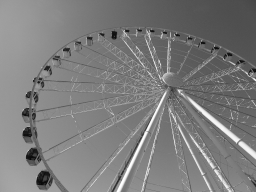
\includegraphics[scale=\myscale,scale=0.7]{figures/image_flou_avant}
	
	Image originale
	\end{minipage}
	\begin{minipage}{0.45\textwidth}\center
	 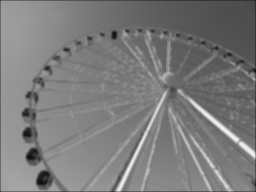
\includegraphics[scale=\myscale,scale=0.7]{figures/image_flou_apres}
	
	Flou
    \end{minipage}	
\end{center}


En effet, la convolution par cette matrice $M$ remplace la couleur d'un pixel par la moyenne de la couleur de ses $9$ pixels voisins. 
Outre l'aspect esthétique, il y a un intérêt fondamental : le flou réduit le bruit. 
Par exemple, si un pixel est mauvais (par exemple à cause d'une erreur de l'appareil photo), le flou élimine cette erreur.

Une variante est le \emph{flou gaussien} défini par la matrice :
$$M = 
\frac{1}{16} \begin{pmatrix}
1&2&1\\
2&4&2\\
1&2&1
\end{pmatrix}.$$
Il existe aussi des flous définis par des matrices $M$ de taille $5 \times 5$, qui tiennent compte des $25$ pixels voisins.


%--------------------------------------------------------------------
\subsection{Piqué}

C'est en quelque sorte le contraire du flou ! Le motif est : 

$$M = 
\begin{pmatrix}
0&-1&0\\
-1&5&-1\\
0&-1&0\\
\end{pmatrix}.$$

Voici un exemple avec l'image originale à gauche et l'image transformée à droite qui a l'air plus nette que l'originale !

\begin{center}
	\begin{minipage}{0.45\textwidth}\center
       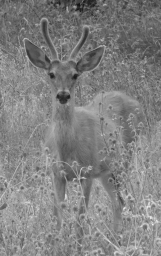
\includegraphics[scale=\myscale,scale=0.7]{figures/image_pique_avant}
	
	Image originale
	\end{minipage}
	\begin{minipage}{0.45\textwidth}\center
	 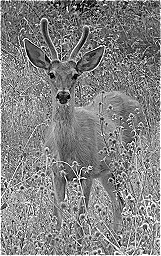
\includegraphics[scale=\myscale,scale=0.7]{figures/image_pique_apres}
	
	Piqué
    \end{minipage}	
\end{center}

%--------------------------------------------------------------------
\subsection{Verticales et horizontales}

Le motif suivant renforce les lignes verticales :
$$M = 
\begin{pmatrix}
-1&2&-1\\
-1&2&-1\\
-1&2&-1\\
\end{pmatrix}.$$

\begin{center}
	\begin{minipage}{0.45\textwidth}\center
       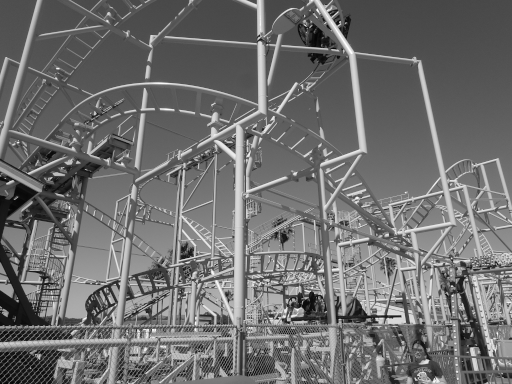
\includegraphics[scale=\myscale,scale=0.4]{figures/image_verticales_avant}
	
	Image originale
	\end{minipage}
	\begin{minipage}{0.45\textwidth}\center
	 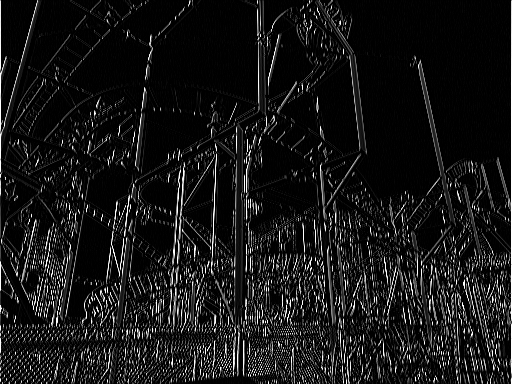
\includegraphics[scale=\myscale,scale=0.4]{figures/image_verticales_apres}
	
	Verticales
    \end{minipage}	
\end{center}

De même pour les lignes horizontales (à gauche) ou les lignes à $45^\circ$ (à droite) :
$$M = 
\begin{pmatrix}
-1&-1&-1\\
2&2&2\\
-1&-1&-1\\
\end{pmatrix},\qquad \qquad
M=\begin{pmatrix}
-1&-1&2\\
-1&2&-1\\
2&-1&-1\\
\end{pmatrix}.
$$

\begin{center}
	\begin{minipage}{0.45\textwidth}\center
	 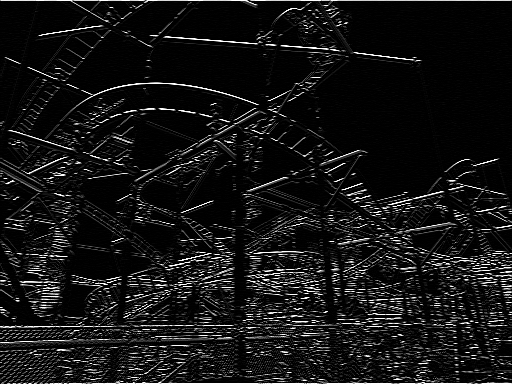
\includegraphics[scale=\myscale,scale=0.4]{figures/image_horizontales_apres}
	
	Horizontales
    \end{minipage}
	\begin{minipage}{0.45\textwidth}\center
	 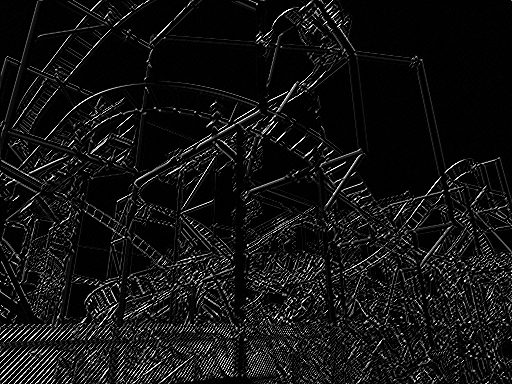
\includegraphics[scale=\myscale,scale=0.4]{figures/image_diagonales_apres}
	
	Diagonales
    \end{minipage}        	
\end{center}


Ce que l'on retient, c'est que la convolution permet de détecter des lignes verticales ou horizontales par exemple et donc d'extraire des caractéristiques abstraites d'une image.

%--------------------------------------------------------------------
\subsection{Bords}

On peut plus généralement extraire les bords des formes d'une image avec : 

$$M = 
\begin{pmatrix}
-1&-1&-1\\
-1&8&-1\\
-1&-1&-1\\
\end{pmatrix}.$$


\begin{center}
	\begin{minipage}{0.45\textwidth}\center
       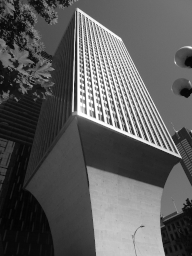
\includegraphics[scale=\myscale,scale=0.7]{figures/image_contour_avant}
	
	Image originale
	\end{minipage}
	\begin{minipage}{0.45\textwidth}\center
	 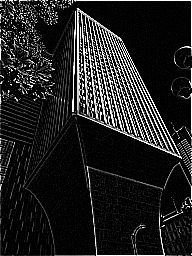
\includegraphics[scale=\myscale,scale=0.7]{figures/image_contour_apres}
	
	Contour
    \end{minipage}	
\end{center}

Des variantes sont les matrices : 
$$M = 
\begin{pmatrix}
0&1&0\\
1&-4&1\\
0&1&0\\
\end{pmatrix} \qquad \text{ ou } \qquad
M = \begin{pmatrix}
1&0&-1\\
0&0&0\\
-1&0&1\\
\end{pmatrix}.$$


%--------------------------------------------------------------------
\subsection{Mise en relief}

En jouant sur les contrastes, on peut créer une impression de relief avec : 

$$M = 
\begin{pmatrix}
-2&-1&0\\
-1&1&1\\
0&1&2\\
\end{pmatrix}.$$

\begin{center}
	\begin{minipage}{0.45\textwidth}\center
       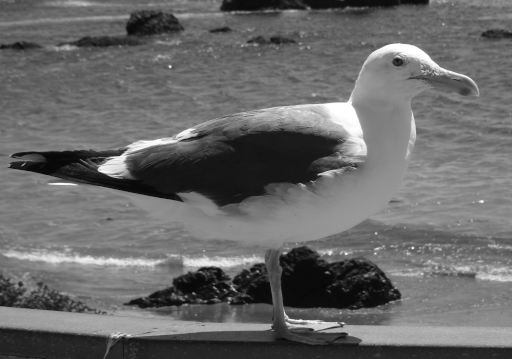
\includegraphics[scale=\myscale,scale=0.4]{figures/image_relief_avant}
	
	Image originale
	\end{minipage}
	\begin{minipage}{0.45\textwidth}\center
	 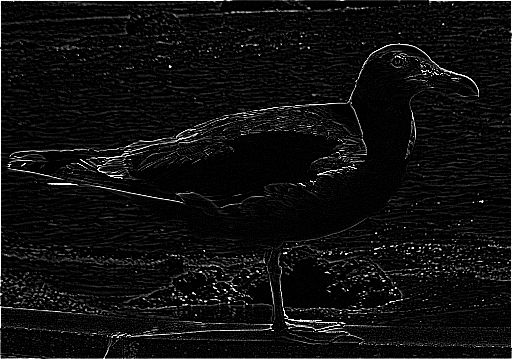
\includegraphics[scale=\myscale,scale=0.4]{figures/image_relief_apres}
	
	Relief
    \end{minipage}	
\end{center}


%--------------------------------------------------------------------
\subsection{Pooling}

On termine cette section en illustrant l'action du pooling sur une image.

\begin{center}
	\begin{minipage}{0.45\textwidth}\center
       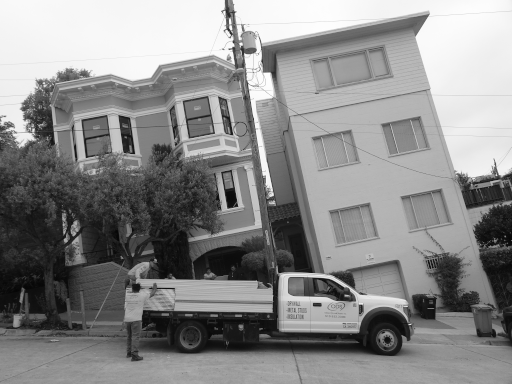
\includegraphics[scale=\myscale,scale=0.4]{figures/image_pooling_avant}
	
	Image originale
	\end{minipage}
	\begin{minipage}{0.2\textwidth}\center
	 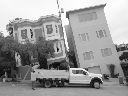
\includegraphics[scale=\myscale,scale=0.4]{figures/image_pooling_max}
	
	Max-pooling $4\times 4$
    \end{minipage}
	\begin{minipage}{0.2\textwidth}\center
	 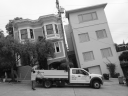
\includegraphics[scale=\myscale,scale=0.4]{figures/image_pooling_average}
	
	Pooling $4\times 4$ en moyenne
    \end{minipage}    
\end{center}

Les images obtenues comportent $16$ fois moins de pixels. Les voici agrandies.

\begin{center}
	\begin{minipage}{0.45\textwidth}\center
	 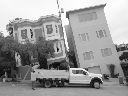
\includegraphics[scale=\myscale,scale=1.6]{figures/image_pooling_max}
	
	Max-pooling $4\times 4$
    \end{minipage}
	\begin{minipage}{0.45\textwidth}\center
	 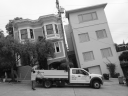
\includegraphics[scale=\myscale,scale=1.6]{figures/image_pooling_average}
	
	Pooling $4\times 4$ en moyenne
    \end{minipage}    
\end{center}

%%%%%%%%%%%%%%%%%%%%%%%%%%%%%%%%%%%%%%%%%%%%%%%%%%%%%%%%%%%%%%%%%%%%%
\section{Rétropropagation}

\index{retropropagation@rétropropagation}
\index{descente de gradient!retropropagation@rétropropagation}

Les formules de la rétropropagation s'étendent sans problème au cas des neurones de convolution.
On commence par reprendre les calculs du chapitre \og{}Gradient\fg{} pour le cas classique avant de s'occuper du cas de la convolution.

\textbf{Cas classique.}

Voici la situation d'un neurone. On ne s'intéresse qu'à une seule de ses arêtes d'entrée : celle associée au poids $a$ et de valeur d'entrée $f$. 
Ce neurone a pour fonction d'activation $g$. La sortie de ce neurone est utilisée par le reste du réseau. À la fin, on obtient une valeur de sortie pour la fonction $F$.

   \myfigure{0.8}{
   \tikzinput{fig-conv-retro-01}
   } 


On distingue la fonction de sa valeur en un point : on note $f$ la fonction et $f_\mystar$ la valeur de la fonction à la sortie du neurone correspondant. De même pour $g$ et $g_\mystar$ et la valeur de la dérivée $g'_\mystar$.

   \myfigure{0.8}{
   \tikzinput{fig-conv-retro-02}
   } 


On reprend la formule du chapitre \og{}Gradient\fg{}:
$$\frac{\partial F}{\partial a} = \frac{\partial F}{\partial g} \cdot f_\mystar \cdot  g'_\mystar.$$

Nous avions vu comment cette formule permettait de calculer le gradient par rapport aux poids.


\emph{Preuve.}
Tour d'abord $$\frac{\partial F}{\partial a} =  \frac{\partial F}{\partial g} \cdot \frac{\partial g}{\partial a}.$$
Or 
$$\frac{\partial g}{\partial a} = f_\mystar \cdot g'_\mystar$$
car 
$g_\mystar = g(\cdots + a f_\mystar+\cdots)$. La formule s'obtient en dérivant $a \mapsto g(\cdots + a f +\cdots)$ par rapport à la variable $a$.

\textbf{Cas de la convolution.}

On se place maintenant dans une couche de convolution. Les neurones de cette couche ont des poids en commun, il faut donc en tenir compte dans les formules.
Imaginons une couche de convolution avec deux neurones.

   \myfigure{0.8}{
   \tikzinput{fig-conv-retro-03}
   } 


Ces deux neurones ont un poids commun $a$, par contre les entrées pour ce poids 
$f_{1,\mystar}$ et $f_{2,\mystar}$ peuvent être différentes et les sorties $g_{1,\mystar}$ et $g_{2,\mystar}$ également (même si les fonctions d'activation $g_1$ et $g_2$ sont les mêmes).
Le réseau continue. À la fin, nous obtenons un fonction de sortie $F$ qui dépend des sorties $g_1$ et $g_2$ de nos deux neurones  :
$$F = \psi(g_1,g_2).$$

   \myfigure{0.8}{
   \tikzinput{fig-conv-retro-04}
   } 

Nous avons la nouvelle formule :
$$\frac{\partial F}{\partial a} = \frac{\partial F}{\partial g_1} \cdot f_{1,\mystar} \cdot  g'_{1,\mystar} + \frac{\partial F}{\partial g_2} \cdot f_{2,\mystar} \cdot  g'_{2,\mystar}.$$


\emph{Preuve.}
Tout d'abord nous avons $F = \psi(g_1,g_2)$, donc
$$\frac{\partial F}{\partial g_1} = \frac{\partial \psi}{\partial x}(g_1,g_2)
\quad\text{ et }\quad
\frac{\partial F}{\partial g_2} = \frac{\partial \psi}{\partial y}(g_1,g_2).$$


On se souvient de la formule de dérivation de la composition de
$$F(a) = \psi\big( u(a), v(a) \big)$$
qui est 
$$F'(a) = u'(a) \frac{\partial \psi}{\partial x}(u(a),v(a)) \  + \  v'(a) \frac{\partial \psi}{\partial y}(u(a),v(a)).$$

Comme on peut aussi écrire que :
$$F = \psi\big( g_1(\cdots + af_1+\cdots) , g_2(\cdots + af_2+\cdots) \big)$$
alors

\begin{align*}
\frac{\partial F}{\partial a} =
f_1 \cdot g_1'(\cdots + af_1+\cdots) \frac{\partial \psi}{\partial x}\big( g_1(\cdots + af_1+\cdots) , g_2(\cdots + af_2+\cdots)\big) \\
+ 
f_2 \cdot g_2'(\cdots + af_1+\cdots) \frac{\partial \psi}{\partial y}\big( g_1(\cdots + af_1+\cdots) , g_2(\cdots + af_2+\cdots)\big).
\end{align*}

Ce qui donne bien :
$$\frac{\partial F}{\partial a} =
f_{1,\mystar} \cdot g'_{1,\mystar} \cdot \frac{\partial F}{\partial g_1}
+ 
f_{2,\mystar} \cdot g'_{2,\mystar} \cdot \frac{\partial F}{\partial g_2}.
$$


Si les fonctions d'activation de la couche de convolution sont l'identité alors $g'_{1,\mystar} = 1$ et $g'_{2,\mystar} = 1$, on obtient dans ce cas la formule :
$$\frac{\partial F}{\partial a} =
f_{1,\mystar} \cdot \frac{\partial F}{\partial g_1}
+ 
f_{2,\mystar} \cdot \frac{\partial F}{\partial g_2}.$$

On retient que chaque entrée associée au poids $a$ contribue proportionnellement à sa valeur dans le calcul de la dérivée partielle par rapport à ce poids $a$.

Plus généralement, pour des entrées $f_i$, $i=1,\ldots,n$, pour $n$ neurones d'une couche de convolution ayant pour sortie $g_i$, $i=1,\ldots,n$, et pour un poids $a$ partagé par ces neurones :
$$\frac{\partial F}{\partial a} = \sum_{i=1}^n f_{i,\mystar} \cdot g'_{i,\mystar} \cdot \frac{\partial F}{\partial g_i}.$$
\end{document}
